% apresentacao_cgs_sat_main.tex  (pack: apresentacao_cgs_sat_main_rob_v1)
% Beamer — CGS sat-main + robustez de amostra (FE_MAIN = PRINCIPAL).
% Números principais: REMODELADO_sat_main_v1/ (copiados do pack v3).
% Números de robustez: REMODELADO_sat_main_rob_v1/ (semF + cnae2).
% FE_MAIN: classe×mês_cal + município×time_id + classe×município×mês_cal + município×ano
%          δ_{s,c(t)} + μ_{mt} + α_{sm,c(t)} + γ_{m,year(t)}
% mês_cal = calendário 1–12; time_id = mês civil (competência).
% D_s ∈ {0,1} binary listed. No class×year / class×time. Lean FE = comparison only.
% Oral spine: RQ → design → Saturar → ATT+p → Δ/5 → ES W_sk → binary+T_max → robustez (cortes) → null.
% NÃO sobrescreve apresentacao_cgs_sat_main_v3.
% Compile: pdflatex ×2.
\documentclass[aspectratio=169,11pt]{beamer}
\usetheme{default}
\usecolortheme{default}
\setbeamertemplate{navigation symbols}{}
\setbeamertemplate{footline}[frame number]
\setbeamerfont{frametitle}{series=\bfseries,size=\large}
\setbeamerfont{title}{series=\bfseries,size=\Large}
\usepackage{amsmath,amssymb,booktabs,graphicx,array,tabularx}
\graphicspath{{./}{figuras/}}
\usepackage[T1]{fontenc}
\usepackage[utf8]{inputenc}
\newcommand{\Ds}{D_s}
% Compact cell: coef / (se) / [p]
\newcommand{\csp}[3]{\begin{tabular}{@{}c@{}}#1\\{\scriptsize(#2)}\\{\scriptsize[#3]}\end{tabular}}
\title{Reoneração gradual da folha e o mercado de trabalho formal}
\subtitle{Evidências da Lei n\textsuperscript{o} 14.973/2024 --- CGS sat-main + robustez (rob\_v1)}
\author{Victor Moreschi}
\institute{Causal Inference II --- Prof.\ Cristine Campos de Xavier Pinto}
\date{Outubro de 2026}

\begin{document}

\begin{frame}[plain]
  \titlepage
\end{frame}

\begin{frame}{Roteiro (oral)}
\tableofcontents[sections={1-5}]
\end{frame}

% ============================================================
\section{Pergunta}
% ============================================================
\begin{frame}{Pergunta de pesquisa}
O cronograma de reoneração de 2025--26 alterou o \textbf{saldo} de emprego formal
(ou admissões / desligamentos) nas classes CNAE listadas, frente a classes que já
pagavam 20\% de CPP?
\begin{itemize}
  \item Literatura mediu \emph{desoneração} (efeitos fracos/nulos).
  \item Aqui medimos a \emph{saída} do benefício, na rampa estatutária \(0/5/10\).
  \item Identificação setorial e contemporânea: toda classe listada enfrenta o mesmo calendário.
\end{itemize}
\end{frame}

% ============================================================
\section{Desenho}
% ============================================================
\begin{frame}{Contexto --- Lei 14.973/2024}
\begin{center}
\begin{tabular}{ccc}
\toprule
Ano & CPP sobre a folha & CPRB sobre a receita \\
\midrule
2024 & 0\% & alíquota cheia (1--4,5\%) \\
2025 & 5\% & 80\% da alíquota cheia \\
2026 & 10\% & 60\% da alíquota cheia \\
2027 & 15\% & 40\% da alíquota cheia \\
2028-- & 20\% & extinta \\
\bottomrule
\end{tabular}
\end{center}
\vspace{0.5em}
Jan/2023--jun/2026. Contraste: listada em 2025 (dose~5) e em 2026 (dose~10) vs base 2023--24.\\
Parâmetro: ITT setorial (CAGED não separa híbrido vs 20\% vs Simples).
\end{frame}

\begin{frame}{Painel e FE\_MAIN (saturados = principais)}
\begin{itemize}
  \item Célula: classe CNAE \(\times\) município \(\times\) mês; zeros onde o CAGED é silencioso.
  \item \(N=9{,}219{,}210\) fluxos (FE\_MAIN); salário: filtro 0,3--150 SM; drop ago--set/2023 só em wage (\(N=2{,}222{,}824\)).
  \item NEVER\_DROP: 1521, 1529, 4911, 5212, 5231, 5510 (saíram em 2018).
  \item \textbf{FE\_MAIN (preferidos):} classe\(\times\)mês\_cal + município\(\times\)mês civil (\texttt{time\_id}) + classe\(\times\)município\(\times\)mês\_cal + município\(\times\)ano.\\
        Em símbolos: \(\delta_{s,c(t)}+\mu_{mt}+\alpha_{sm,c(t)}+\gamma_{m,\mathrm{year}(t)}\).\\
        {\footnotesize mês\_cal = mês do calendário 1--12; time\_id = mês civil (competência).}
  \item \(\delta_{s,c(t)}\) (classe\(\times\)mês\_cal) \textbf{aninha} no triple \(\alpha_{sm,c(t)}\) (listar ambos é intencional para a banca).
  \item UF\(\times\)time\_id / estado\(\times\)mês civil \textbf{omitido} por colinearidade com município\(\times\)time\_id.
  \item Lean FE (\(cnae4\times mes\_cal + municipio + time\_id\)) = \textbf{comparação apenas}.
  \item Cluster: cnae4. Proibido: classe\(\times\)ano, classe\(\times\)time\_id, classe\(\times\)2025/2026 (absorvem \(\beta_5/\beta_{10}\)).
\end{itemize}
\end{frame}

\begin{frame}{Saturar a dose --- \(\beta_5\) e \(\beta_{10}\) | FE\_MAIN}
Rampa legal \(0/5/10\) nas listadas; saturação = \textbf{dois dummies anuais}
\(\times\) tratado binário (não uma reta em Dose):
\begin{equation*}
\begin{aligned}
Y_{smt}
&=
\delta_{s,c(t)}+\mu_{mt}+\alpha_{sm,c(t)}+\gamma_{m,\mathrm{year}(t)} \\
&\quad
+\beta_5\,\Ds\cdot\mathbf{1}\{t\in 2025\}
+\beta_{10}\,\Ds\cdot\mathbf{1}\{t\in 2026\}
+\varepsilon_{smt}.
\end{aligned}
\end{equation*}
{\footnotesize FE\_MAIN: \(\delta\) = classe\(\times\)mês\_cal; \(\mu\) = município\(\times\)mês civil (\texttt{time\_id});
\(\alpha\) = classe\(\times\)município\(\times\)mês\_cal; \(\gamma\) = município\(\times\)ano.
classe\(\times\)mês\_cal aninha no triple; UF\(\times\)time omitido.}
\begin{itemize}
  \item \(\Ds\in\{0,1\}\): classe \emph{listada} (binário). Não é a dose \(\{0,5,10\}\).
  \item Base omitida: 2023--2024. \(\beta_5\): ATT em 2025 vs base; \(\beta_{10}\): ATT em 2026 vs \emph{mesma} base.
  \item Proibido: classe\(\times\)ano, classe\(\times\)time\_id, classe\(\times\)2025/2026 (absorvem \(\beta_5/\beta_{10}\)).
  \item \(\delta_{s,c(t)}\) \textbf{aninha} em \(\alpha_{sm,c(t)}\) (listar ambos intencional); UF\(\times\)time omitido por colinearidade com \(\mu_{mt}\).
  \item As interações \textbf{engolem} os FE simples (classe, município, mês): escrevê-los de novo seria colinear.
  \item Reta linear em Dose = coluna de comparação apenas.
\end{itemize}
\end{frame}

% ============================================================
\section{Resultados principais}
% ============================================================
\begin{frame}{Tabela principal --- ATTs anuais (FE\_MAIN; saldo em destaque)}
\begin{center}
\scriptsize
\setlength{\tabcolsep}{3.5pt}
\begin{tabular}{lccc}
\toprule
Outcome & \(\hat\beta_5\) & \(\hat\beta_{10}\) & \(\widehat{\Delta}/5\) \\
\midrule
\textbf{Saldo}
  & \csp{\textbf{0.020}}{\textbf{0.043}}{\textbf{0.64}}
  & \csp{\textbf{0.011}}{\textbf{0.062}}{\textbf{0.86}}
  & \csp{\textbf{$-$0.0017}}{\textbf{0.013}}{\textbf{0.89}} \\[1.6em]
Admissões
  & \csp{0.001}{0.147}{0.99}
  & \csp{$-$0.112}{0.243}{0.65}
  & \csp{$-$0.023}{0.024}{0.35} \\[1.6em]
Desligamentos
  & \csp{$-$0.019}{0.171}{0.91}
  & \csp{$-$0.123}{0.240}{0.61}
  & \csp{$-$0.021}{0.017}{0.23} \\[1.6em]
Log salário adm.
  & \csp{$-$0.0010}{0.0018}{0.58}
  & \csp{$-$0.0017}{0.0027}{0.54}
  & \csp{$-$0.0001}{0.0003}{0.71} \\
\bottomrule
\end{tabular}
\end{center}
\vspace{0.35em}
{\footnotesize Células: coef / (s.e.) / [\(p\)]. FE\_MAIN; cluster cnae4.\\
Fluxos \(N=9{,}219{,}210\); wage \(N=2{,}222{,}824\). Fonte: \texttt{tab\_att\_principal\_wide\_for\_tex.csv}.\\
\(\widehat{\Delta}=\hat\beta_{10}-\hat\beta_5\): saldo $-$0.0087 (0.065) [\(p=0.89\)].}
\end{frame}

\begin{frame}{\((\beta_{10}-\beta_5)/5\) --- leitura cautelosa}
Sob hipótese forte (CGS Thm 3.3(d)), \(\widehat{\Delta}/5\) seria ACRT de um ponto entre dose~5 e~10.\\
Sem ela, o contraste mistura incremento de dose e seleção.
\begin{itemize}
  \item Invocamos a leitura forte porque a lei atribui 5 e depois 10 às \emph{mesmas} classes.
  \item Caveat: 2026 já carrega um ano sob dose~5; dinâmicas permanecem.
  \item Reportamos \(\widehat{\Delta}/5\approx -0.0017\) (s.e.\ 0.013, \(p\approx 0.89\)) \textbf{com} esse parágrafo.
  \item \textbf{Não} declaramos ACRT limpo; \textbf{não} validamos SPT; \textbf{não} usamos \(\beta_5/5=\beta_{10}/10\).
\end{itemize}
\end{frame}

\begin{frame}{ES preferido --- dose \(W_{sk}\), saldo (FE\_MAIN)}
\begin{center}
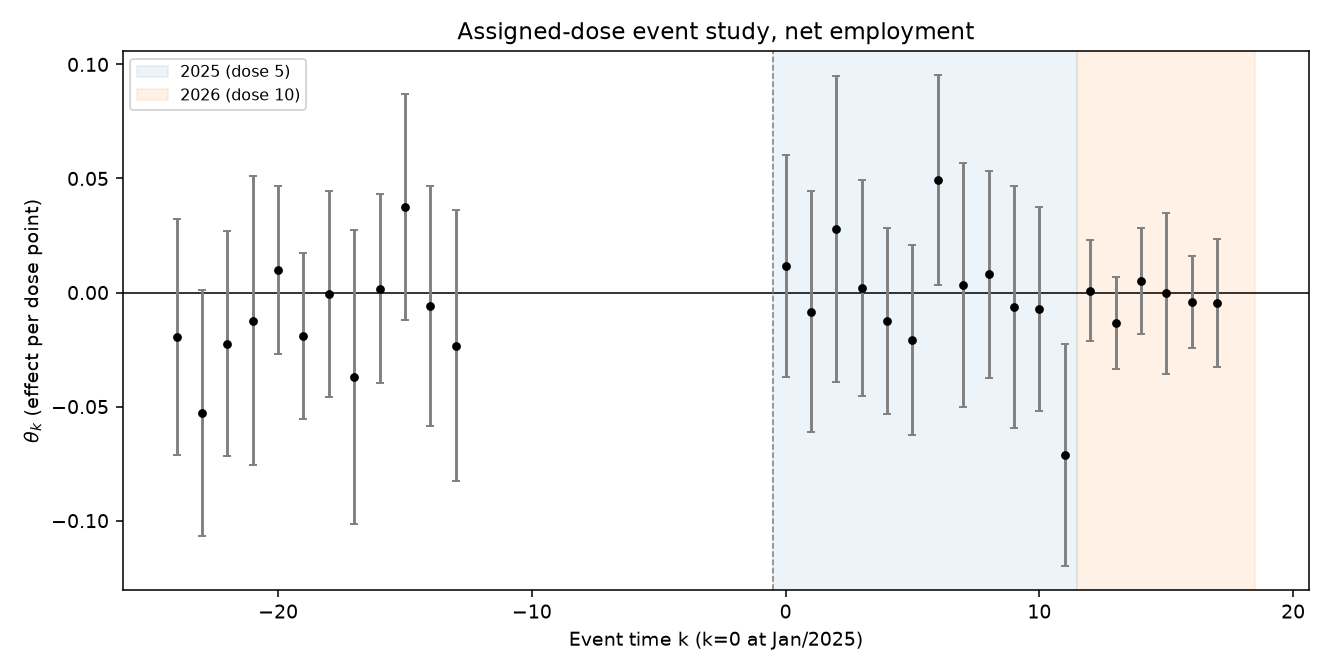
\includegraphics[width=0.92\textwidth,height=0.58\textheight,keepaspectratio]{fig_es_dose_base2024_saldo.png}
\end{center}
\vspace{-0.2em}
{\footnotesize \(W=0\) controle; \(W=5\) listada 2023--25; \(W=10\) listada 2026. Pré \(W=5\) = escala do lead, não dose calendário.\\
Base 2024 omitida. Joint \(\theta_k=0\) em 2023: Wald \(\approx 13.3\), \(p\approx 0.35\) (implicação comum; \(\neq\) aceite SPT). FE\_MAIN.}
\end{frame}

\begin{frame}{ES binário + \(T_{\max}\) (PT usual | FE\_MAIN)}
\begin{columns}[T]
\begin{column}{0.58\textwidth}
\centering
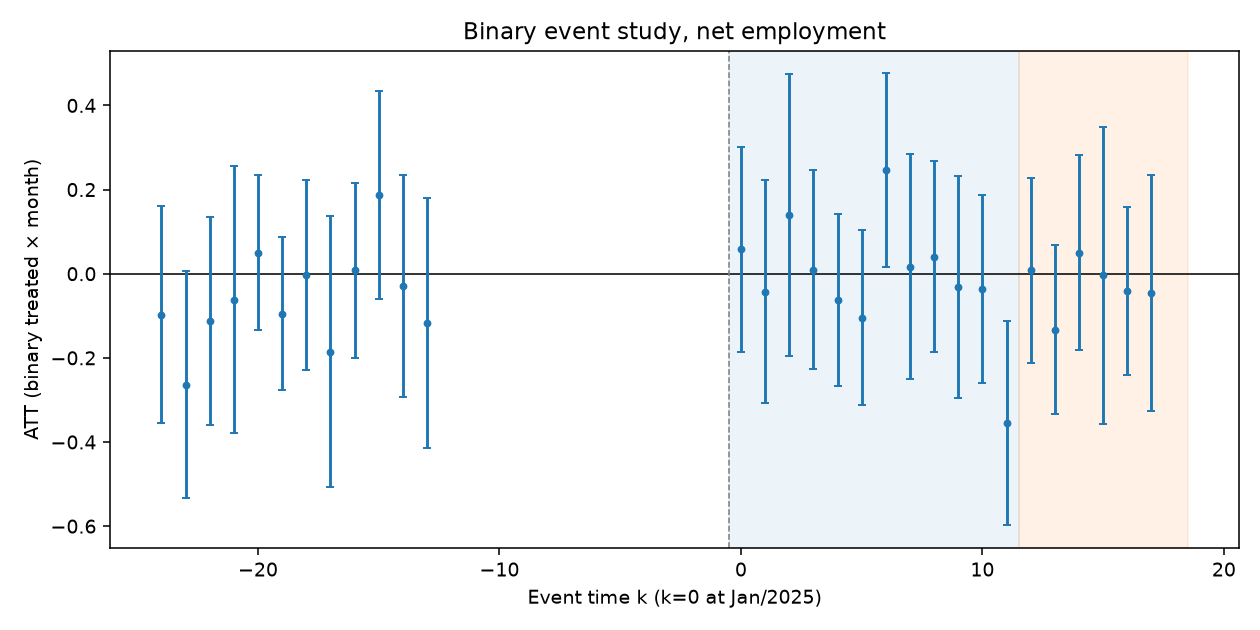
\includegraphics[width=\textwidth]{fig_es_binario_base2024_saldo.png}
\end{column}
\begin{column}{0.40\textwidth}
\small
Timing de exposição, \textbf{não} preferido.\\[0.5em]
\(T_{\max}\) nos 12 leads de 2023 (saldo):\\
\(T_{\max}\approx 1.92\), crit.\ 5\% \(\approx 2.82\), \(p\approx 0.43\).\\[0.5em]
= PT usual em \(Y(0)\), \textbf{não} SPT.\\[0.6em]
{\footnotesize Ambos ES (dose-\(W\) e binário) sob FE\_MAIN.}
\end{column}
\end{columns}
\end{frame}

% ============================================================
\section{Robustez}
% ============================================================
\begin{frame}{Robustez --- dois cortes de amostra (mesma FE\_MAIN)}
\small
Mesma especificação principal; só muda a amostra. Cluster cnae4.
\begin{enumerate}
  \item \textbf{Principal} --- amostra completa (\(N=9{,}219{,}210\) fluxos). Fonte: \texttt{REMODELADO\_sat\_main\_v1/}.
  \item \textbf{semF} --- drop seção F (construção). \(N=7{,}754{,}460\).
  \item \textbf{cnae2} --- controles restritos a divisões CNAE~2 com \(\geq 1\) classe listada (\(n_{\mathrm{divs}}=27\)). \(N=6{,}294{,}582\).
\end{enumerate}
\vspace{0.4em}
\textbf{FE\_MAIN (igual ao principal):}\\
classe\(\times\)mês\_cal + município\(\times\)time\_id + classe\(\times\)município\(\times\)mês\_cal + município\(\times\)ano\\
\(\equiv\delta_{s,c(t)}+\mu_{mt}+\alpha_{sm,c(t)}+\gamma_{m,\mathrm{year}(t)}\).\\[0.3em]
{\footnotesize mês\_cal = 1--12; time\_id = mês civil. classe\(\times\)mês\_cal aninha no triple; UF\(\times\)time omitido; proibido classe\(\times\)ano/time/2025--26.\\
Números de robustez: \texttt{REMODELADO\_sat\_main\_rob\_v1/}.}
\end{frame}

\begin{frame}{Robustez --- ATT saldo: Principal \(\mid\) semF \(\mid\) cnae2}
\begin{center}
\scriptsize
\setlength{\tabcolsep}{2.8pt}
\begin{tabular}{lccc}
\toprule
 & Principal & semF & cnae2 \\
\midrule
\(\hat\beta_5\)
  & \csp{0.020}{0.043}{0.64}
  & \csp{0.084}{0.055}{0.13}
  & \csp{0.012}{0.044}{0.79} \\[1.5em]
\(\hat\beta_{10}\)
  & \csp{0.011}{0.062}{0.86}
  & \csp{0.026}{0.070}{0.71}
  & \csp{0.071}{0.069}{0.30} \\[1.5em]
\(\widehat{\Delta}/5\)
  & \csp{$-$0.0017}{0.013}{0.89}
  & \csp{$-$0.011}{0.016}{0.47}
  & \csp{0.012}{0.012}{0.32} \\[1.5em]
\(N\) & 9{,}219{,}210 & 7{,}754{,}460 & 6{,}294{,}582 \\
\bottomrule
\end{tabular}
\end{center}
\vspace{0.25em}
{\footnotesize Células: coef / (s.e.) / [\(p\)]. FE\_MAIN; cluster cnae4. Outcome: \textbf{saldo}.\\
Outros \(Y\) (admitidos, desligados, wage) também próximos de nulo nos três cortes.\\
Fonte: \texttt{tab\_att\_rob\_wide\_for\_tex.csv}.}
\end{frame}

\begin{frame}{ES dose-\(W\) saldo --- semF (FE\_MAIN)}
\begin{center}
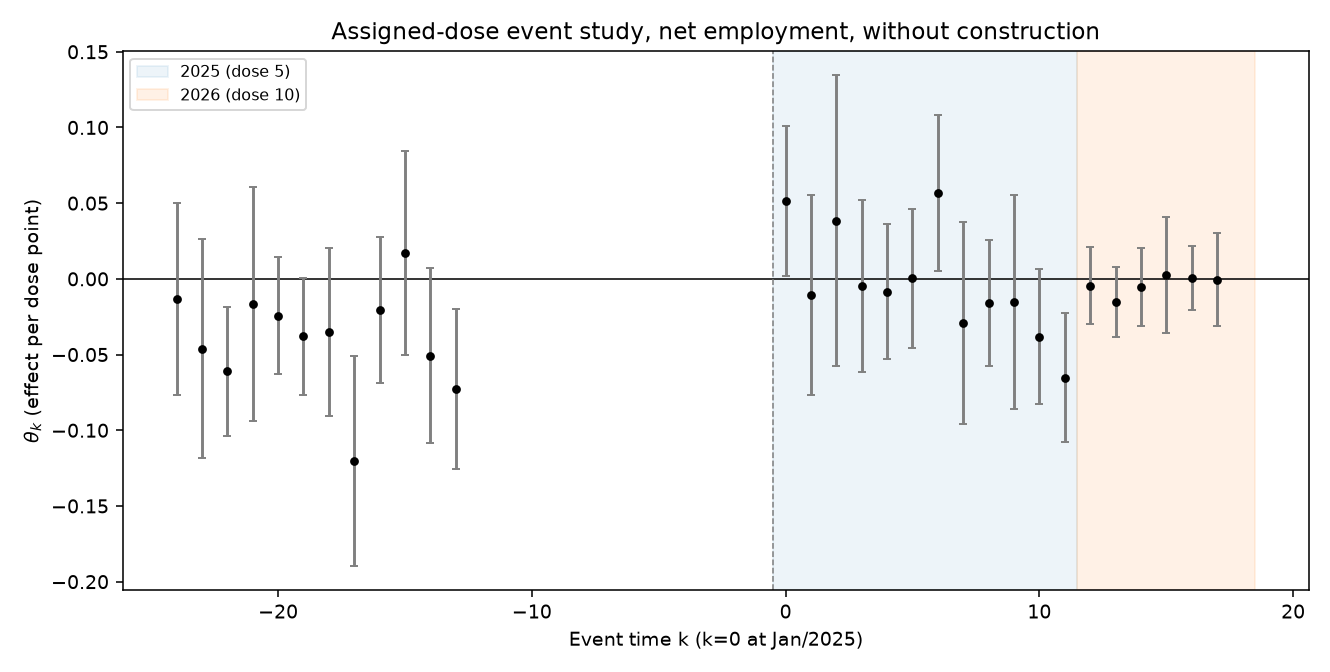
\includegraphics[width=0.92\textwidth,height=0.58\textheight,keepaspectratio]{fig_es_dose_semF_base2024_saldo.png}
\end{center}
\vspace{-0.2em}
{\footnotesize Drop seção F. Spec: \(i(k_{\mathrm{es}})\times W_{sk}\) \(\mid\) FE\_MAIN; base 2024 omitida.\\
ATT saldo ainda nulo-ish (\(\hat\beta_5\approx 0.084\), \(p\approx 0.13\)); ver caveat de \(T_{\max}\) no próximo slide.}
\end{frame}

\begin{frame}{ES dose-\(W\) saldo --- cnae2 (FE\_MAIN)}
\begin{center}
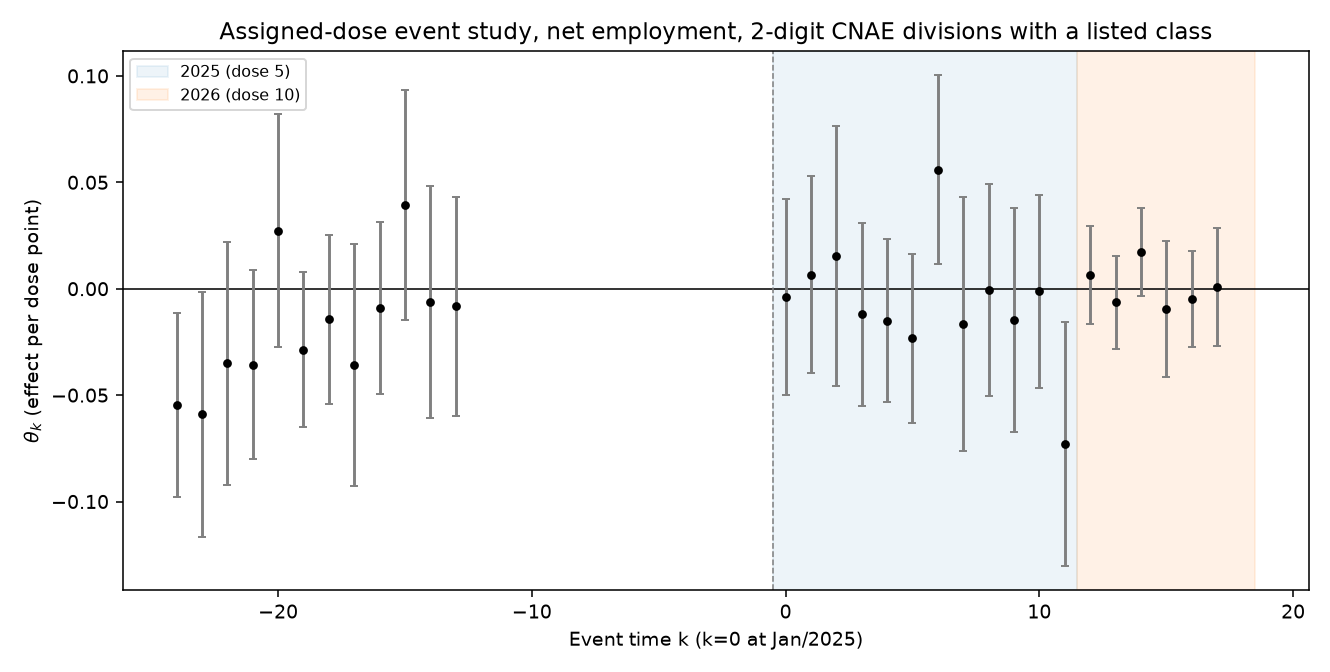
\includegraphics[width=0.92\textwidth,height=0.58\textheight,keepaspectratio]{fig_es_dose_cnae2_base2024_saldo.png}
\end{center}
\vspace{-0.2em}
{\footnotesize Controles em divisões CNAE~2 com listada (\(n_{\mathrm{divs}}=27\)). FE\_MAIN; base 2024.\\
Consistente com o principal: \(\hat\beta_5\approx 0.012\) (\(p\approx 0.79\)), \(\hat\beta_{10}\approx 0.071\) (\(p\approx 0.30\)).}
\end{frame}

\begin{frame}{ES dose-\(W\) admitidos --- semF e cnae2 (apoio)}
\begin{columns}[T]
\begin{column}{0.48\textwidth}
\centering
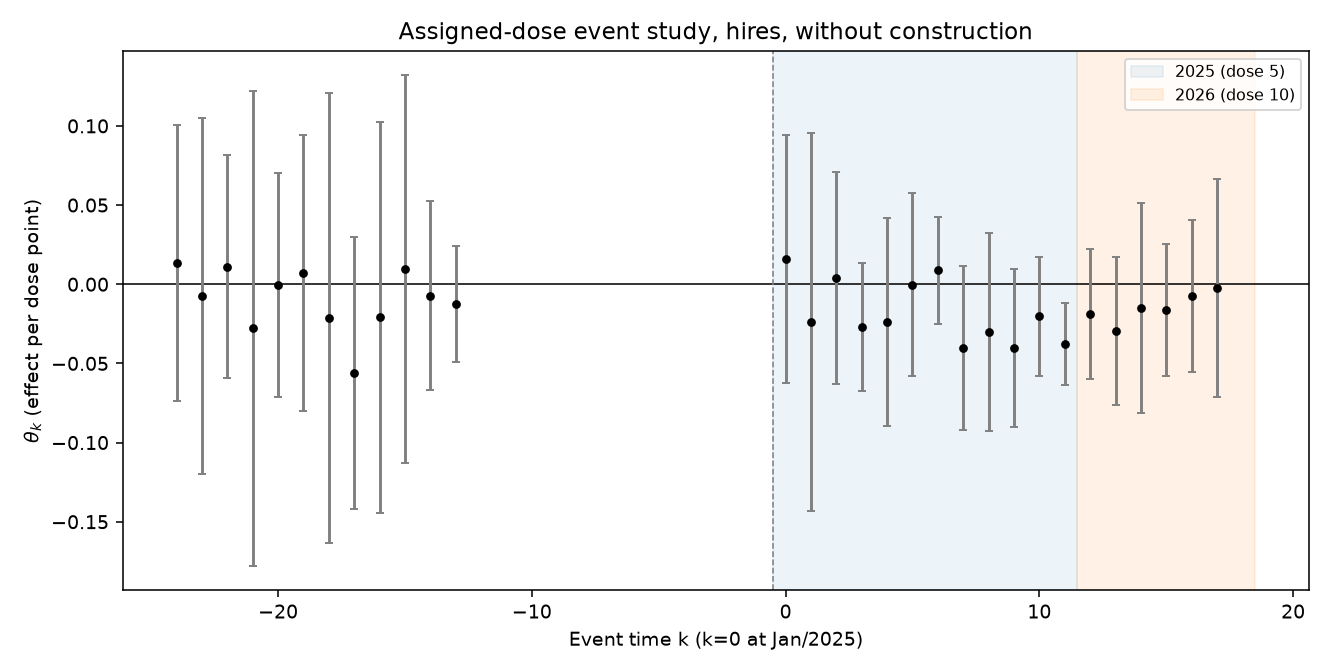
\includegraphics[width=\textwidth]{fig_es_dose_semF_base2024_admitidos.png}\\
{\footnotesize semF --- admitidos}
\end{column}
\begin{column}{0.48\textwidth}
\centering
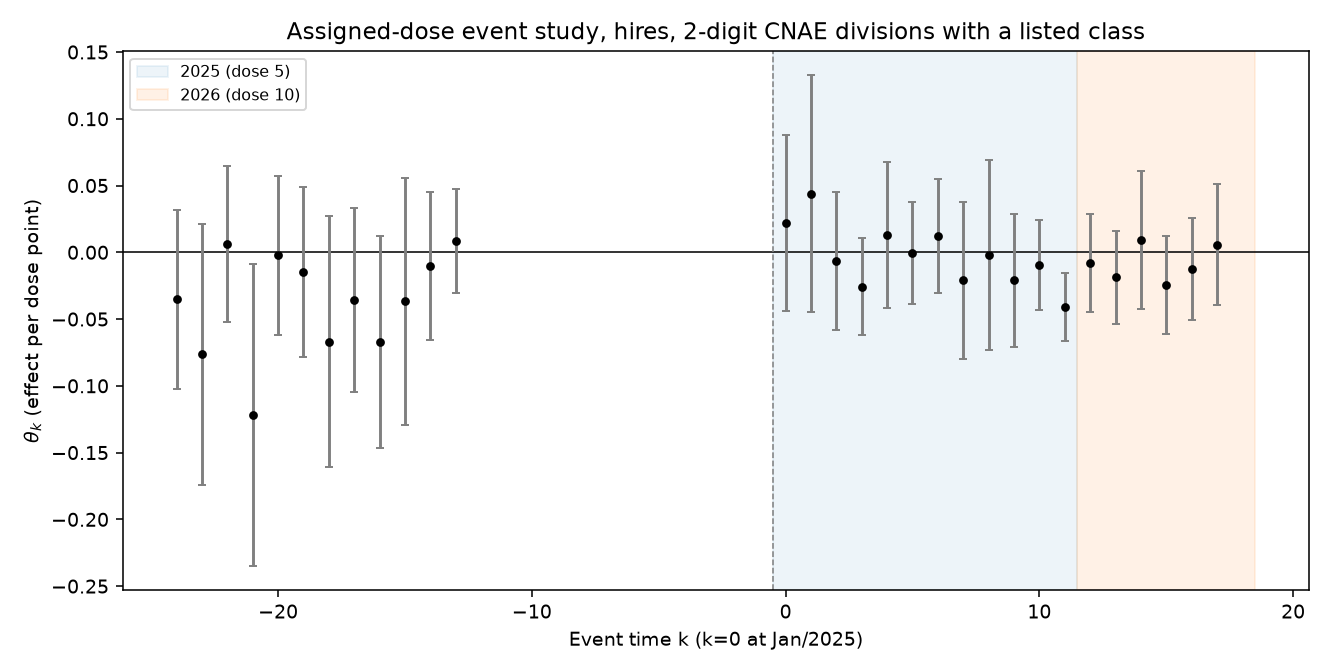
\includegraphics[width=\textwidth]{fig_es_dose_cnae2_base2024_admitidos.png}\\
{\footnotesize cnae2 --- admitidos}
\end{column}
\end{columns}
\vspace{0.2em}
{\footnotesize Apoio; FE\_MAIN; base 2024. Demais \(Y\) (desligados, wage) em backup.}
\end{frame}

\begin{frame}{\(T_{\max}\) / PT usual nos cortes --- caveat semF}
\small
\(T_{\max}\) no ES \textbf{binário} (12 leads de 2023) = \textbf{PT usual} em \(Y(0)\), \textbf{não} SPT.
\begin{center}
\scriptsize
\begin{tabular}{llccc}
\toprule
Corte & Outcome & \(T_{\max}\) & \(p\) & Leitura \\
\midrule
semF & \textbf{saldo} & \textbf{3.40} & \textbf{0.0068} & \textbf{rejeita PT usual} \\
semF & admitidos & 1.28 & 0.54 & OK \\
semF & desligados & 2.24 & 0.10 & marginal \\
semF & log salário & 1.77 & 0.52 & OK \\
\midrule
cnae2 & saldo & 2.47 & 0.13 & não rejeita a 5\% \\
cnae2 & admitidos & 2.11 & 0.14 & OK \\
cnae2 & desligados & 1.63 & 0.36 & OK \\
cnae2 & log salário & 2.10 & 0.30 & OK \\
\bottomrule
\end{tabular}
\end{center}
\vspace{0.3em}
\textbf{Caveat honesto:} em semF, ATT saldo ainda próximo de nulo, mas o PT usual \textbf{falha} no ES binário --- não esconder.\\
cnae2 alinhado ao principal. Fonte: \texttt{tab\_tmax\_semF.csv}, \texttt{tab\_tmax\_cnae2.csv}.
\end{frame}

\begin{frame}{Robustez --- placebo + joint (FE\_MAIN; principal)}
\small
\textbf{Placebo 2024 (FE\_MAIN).} Amostra até dez/2024; ano de tratamento falso = 2024.
\begin{center}
\begin{tabular}{lrrrr}
\toprule
Outcome & coef. & s.e. & \(p\) & \(N\) \\
\midrule
\textbf{Saldo} & \textbf{0.060} & \textbf{0.051} & \textbf{0.24} & 5{,}268{,}120 \\
Admitidos & 0.066 & 0.176 & 0.71 & 5{,}268{,}120 \\
Desligados & 0.006 & 0.170 & 0.97 & 5{,}268{,}120 \\
Log salário & $-$0.0016 & 0.0018 & 0.37 & 886{,}846 \\
\bottomrule
\end{tabular}
\end{center}
\vspace{0.2em}
\textbf{Joint dose-\(W\) 2023 (FE\_MAIN).} Saldo Wald \(\approx 13.3\), \(p\approx 0.35\) (df~12); não-rejeição \(\neq\) aceite SPT.\\[0.3em]
{\footnotesize Comparação (não preferida): lean FE saldo \(\hat\beta_5=0.023\), \(\hat\beta_{10}=0.016\), \(\widehat{\Delta}/5=-0.0015\).\\
Timing placebo sob PT usual, não SPT: não valida hipótese forte nem ACRT.}
\end{frame}

% ============================================================
\section{Conclusão}
% ============================================================
\begin{frame}{Conclusão}
\textbf{Leitura preferida:} nulo setorial de curto prazo no saldo sob FE\_MAIN --- ATTs anuais, não ACRT.
\begin{itemize}
  \item Principal: \(\hat\beta_5\approx 0.020\) (\(p\approx 0.64\)), \(\hat\beta_{10}\approx 0.011\) (\(p\approx 0.86\)); \(T_{\max}\approx 1.92\) (\(p\approx 0.43\)).
  \item \textbf{cnae2:} consistente com o principal (ATT nulo; \(T_{\max}\) saldo \(p\approx 0.13\)).
  \item \textbf{semF:} ATT saldo ainda nulo-ish (\(\hat\beta_5\approx 0.084\), \(p\approx 0.13\)), mas \(T_{\max}\approx 3.40\) (\(p\approx 0.0068\)) \textbf{rejeita PT usual} no ES binário --- divulgar.
  \item \(T_{\max}\) = PT usual, \textbf{não} SPT. Joint pré dose-\(W\) = implicação comum \(\neq\) aceite SPT.
  \item \(\widehat{\Delta}/5\) com hipótese forte; sem ACRT limpo. Wage: caveat de pré frágil.
\end{itemize}
\end{frame}

\begin{frame}{Referências}
\footnotesize
\begin{itemize}
  \item Callaway, B., Goodman-Bacon, A.\ and Sant'Anna, P.\ H.\ C.\ (2024).
        Difference-in-Differences with a Continuous Treatment. NBER WP 32117.
  \item Roth, J., Sant'Anna, P.\ H.\ C., Bilinski, A.\ and Poe, J.\ (2023).
        What's trending in difference-in-differences?
        \emph{Journal of Econometrics} 235, 2218--2244.
  \item Albernaz, L.\ R.\ (2026). Desoneração da folha e emprego formal. Dissertação, IDP.
  \item Reckziegel, B.\ (2024). Desoneração da folha de pagamentos e emprego formal.
\end{itemize}
\end{frame}

% ============================================================
% BACKUP — não oral spine
% ============================================================
\appendix
\section*{BACKUP}

\begin{frame}{BACKUP --- Álgebra de \(\alpha_{sm,c(t)}\) (mês\_cal)}
Fixe classe \(s\), município \(m\) e mês do calendário \(c\) (1--12; ex.: janeiro). \(\alpha_{sm,c}\) = classe\(\times\)município\(\times\)mês\_cal; \emph{não} muda entre anos.\\[0.4em]
O DiD de janeiro usa gaps ano a ano no \emph{mesmo} mês\_cal e município. Após \(\alpha_{sm,c}\), os indicadores de listagem em 2025 e 2026 continuam identificados.\\[0.4em]
\textbf{Mau controle só se} a política mudasse a forma sazonal da classe\(\times\)município.\\
Argumento: sazonalidade (ex.\ construção no Natal) é confounder, não o canal.\\
FE\_MAIN completos: \(\delta_{s,c(t)}+\mu_{mt}+\alpha_{sm,c(t)}+\gamma_{m,\mathrm{year}(t)}\)
(classe\(\times\)mês\_cal aninha no triple; \(\mu_{mt}\) = município\(\times\)mês civil).
\end{frame}

\begin{frame}{BACKUP --- Por que omitir o ano inteiro 2024}
Com \(\alpha_{sm,c(t)}\), um coeficiente de ES é um gap ano a ano no mesmo mês\(\times\)município.\\
Omitir só \(k=-12\) (jan/2024) é a normalização errada.\\[0.4em]
Omitimos o ano-base 2024 inteiro. Pré testável = 2023.\\
Base 2023 deixa 2024 livre --- checagem de antecipação (estatuto: set/2024).
\end{frame}

\begin{frame}{BACKUP --- Definição completa de \(W_{sk}\)}
\begin{itemize}
  \item Controles: \(W=0\) em todos os \(k\).
  \item Listadas em 2023--2025: \(W=5\); listadas em 2026: \(W=10\).
  \item \(\theta_k\) = efeito \textbf{por ponto} naquele mês: \(5\theta_k\approx\) nível 2025; \(10\theta_k\approx\) nível 2026.
  \item Pré \(W=5\) = \textbf{escala do lead} (normalização para o lead não zerar), \textbf{não} dose calendário.
\end{itemize}
\end{frame}

\begin{frame}{BACKUP --- Joint \(\theta_k=0\) em 2023 (dose-\(W\); FE\_MAIN)}
Implicação comum das hipóteses usual e forte (análogo à Fig.~10 CGS).
\begin{center}
\small
\begin{tabular}{lccc}
\toprule
Outcome & Wald & df & \(p\) \\
\midrule
Saldo & 13.30 & 12 & 0.347 \\
Admissões & 14.43 & 12 & 0.274 \\
Desligamentos & 24.08 & 12 & 0.020 \\
Log salário & 18.09 & 10 & 0.053 \\
\bottomrule
\end{tabular}
\end{center}
\vspace{0.4em}
Rejeitar conta contra a implicação comum; \textbf{não rejeitar \(\neq\) aceitar} hipótese forte / SPT.\\
Desligamentos rejeitam; wage \(p\approx 0.05\) --- manter caveat. Fonte: \texttt{tab\_joint.csv}.
\end{frame}

\begin{frame}{BACKUP --- \(T_{\max}\) completo (ES binário; FE\_MAIN)}
\begin{center}
\small
\begin{tabular}{lcccc}
\toprule
Outcome & \(T_{\max}\) & Crit.\ 5\% & \(p\) & \(n_{\mathrm{pre}}\) \\
\midrule
Saldo & 1.92 & 2.82 & 0.43 & 12 \\
Admissões & 1.12 & 2.56 & 0.71 & 12 \\
Desligamentos & 1.48 & 2.57 & 0.42 & 12 \\
Log salário & 1.93 & 2.78 & 0.41 & 10 \\
\bottomrule
\end{tabular}
\end{center}
\vspace{0.4em}
PT usual em \(Y(0)\), não SPT. Fonte: \texttt{tab\_tmax.csv} (FE\_MAIN).
\end{frame}

\begin{frame}{BACKUP --- Reta Dose (comparação; FE\_MAIN)}
\begin{center}
\small
\begin{tabular}{lccc}
\toprule
Outcome & coef & s.e. & \(p\) \\
\midrule
Saldo & 0.0019 & 0.0056 & 0.738 \\
Admissões & $-$0.0081 & 0.0253 & 0.748 \\
Desligamentos & $-$0.0100 & 0.0265 & 0.706 \\
Log salário & $-$0.00018 & 0.00028 & 0.536 \\
\bottomrule
\end{tabular}
\end{center}
\vspace{0.4em}
Impõe linearidade; \textbf{não} é a especificação preferida. Fonte: \texttt{tab\_reta\_comparacao.csv}.
\end{frame}

\begin{frame}{BACKUP --- Lean FE (comparação apenas)}
\begin{center}
\small
\begin{tabular}{lcccc}
\toprule
Outcome & \(\hat\beta_5\) & \(\hat\beta_{10}\) & \(\widehat{\Delta}/5\) & \(N\) \\
\midrule
Saldo & 0.023 & 0.016 & $-$0.0015 & 9{,}221{,}016 \\
Admissões & $-$0.001 & $-$0.112 & $-$0.022 & 9{,}221{,}016 \\
Desligamentos & $-$0.024 & $-$0.127 & $-$0.021 & 9{,}221{,}016 \\
Log salário & $-$0.0009 & $-$0.0023 & $-$0.0003 & 2{,}799{,}714 \\
\bottomrule
\end{tabular}
\end{center}
\vspace{0.4em}
Lean FE \(cnae4\times mes\_cal + municipio + time\_id\) --- \textbf{não} preferida.\\
Fonte: \texttt{tab\_att\_lean\_comparacao.csv}.
\end{frame}

\begin{frame}{BACKUP --- Outros outcomes (apoio; wage com caveat)}
\begin{columns}[T]
\begin{column}{0.48\textwidth}
\centering
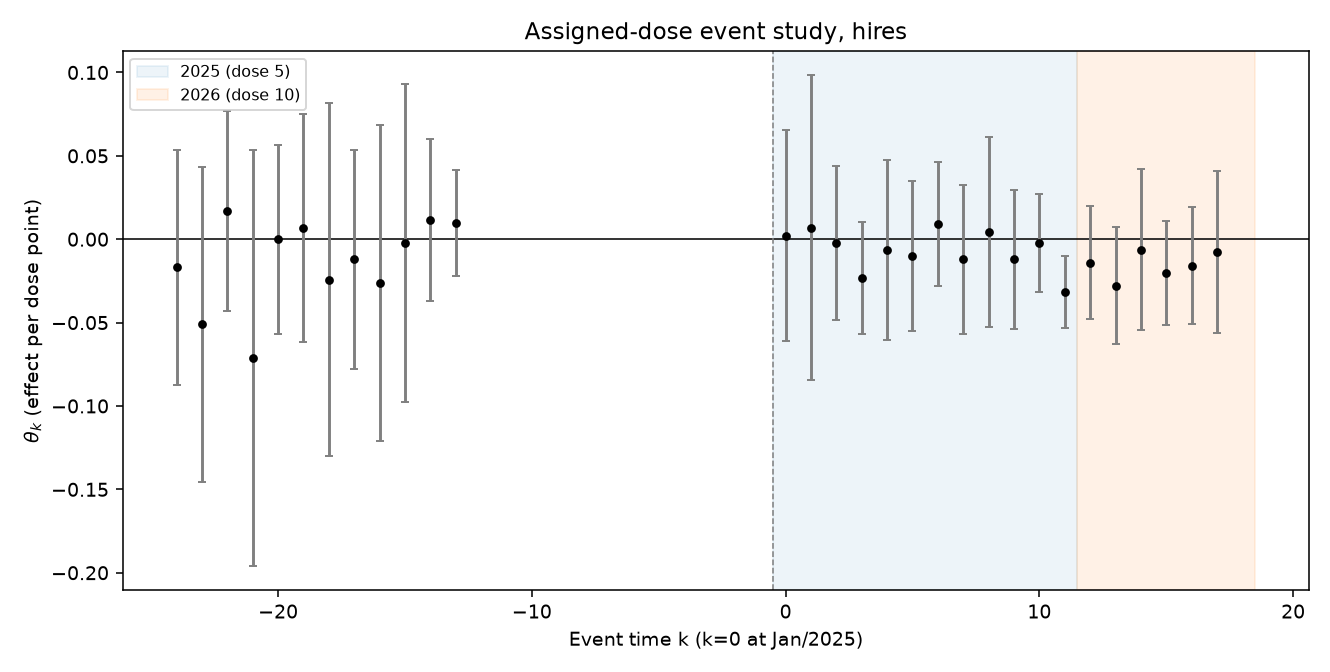
\includegraphics[width=\textwidth]{fig_es_dose_base2024_admitidos.png}\\
{\footnotesize Admissões (apoio; FE\_MAIN)}
\end{column}
\begin{column}{0.48\textwidth}
\centering
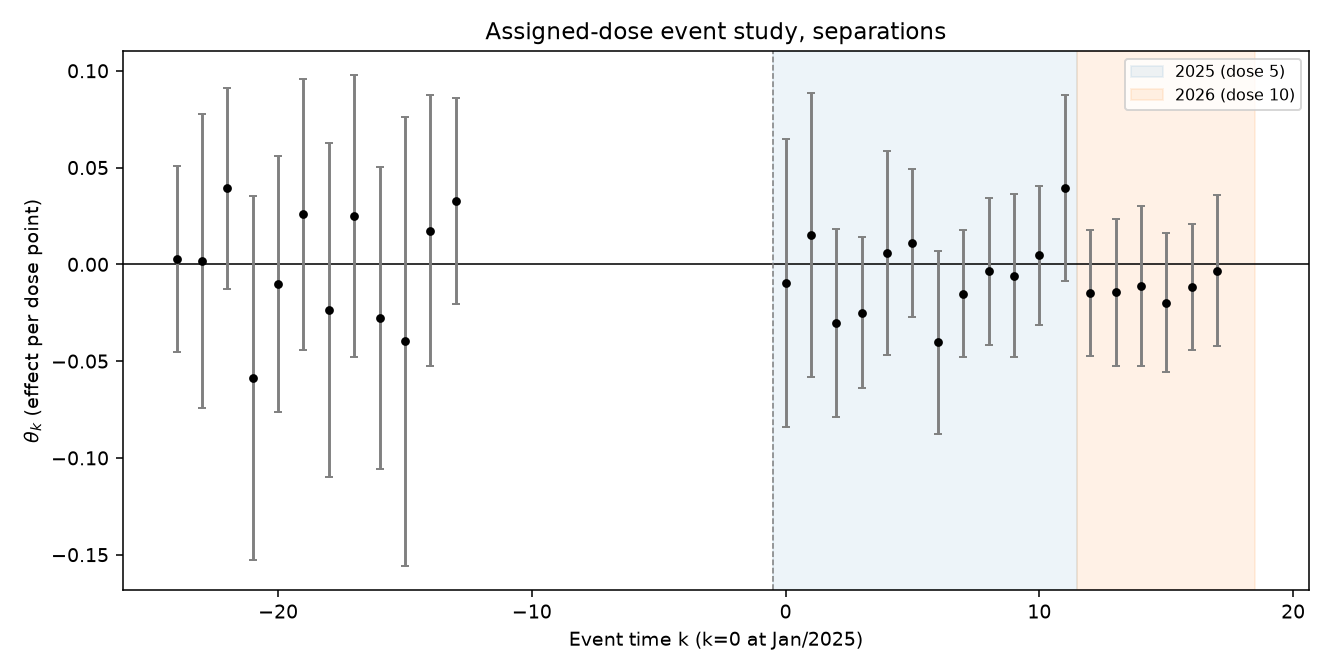
\includegraphics[width=\textwidth]{fig_es_dose_base2024_desligados.png}\\
{\footnotesize Desligamentos (apoio; FE\_MAIN)}
\end{column}
\end{columns}
\end{frame}

\begin{frame}{BACKUP --- Wage ES (pré frágil; não central)}
\begin{center}
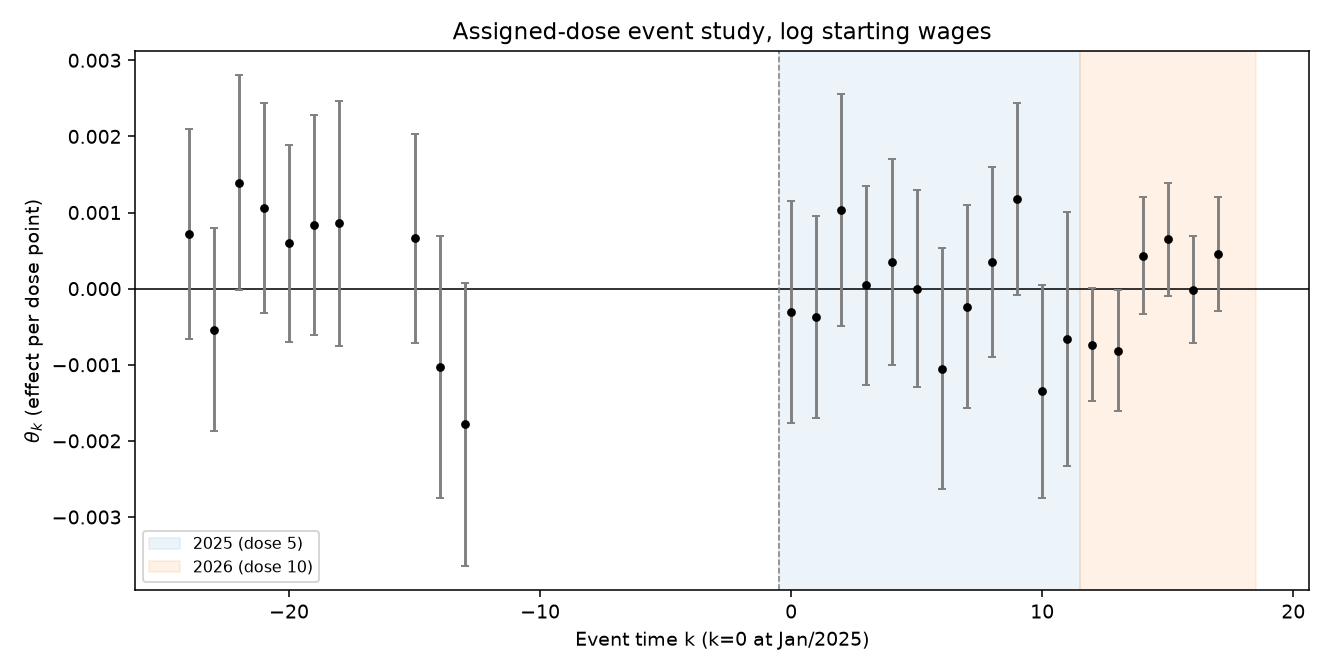
\includegraphics[width=0.85\textwidth,height=0.52\textheight,keepaspectratio]{fig_es_dose_base2024_log_salario.png}
\end{center}
\begin{itemize}
  \item ATTs anuais nulos; joint pré dose-\(W\) \(p\approx 0.053\) (FE\_MAIN).
  \item Não é resultado de apoio ao emprego --- caveat mantido.
\end{itemize}
\end{frame}

\begin{frame}{BACKUP --- ES dose-\(W\) desligados / wage (rob)}
\begin{columns}[T]
\begin{column}{0.48\textwidth}
\centering
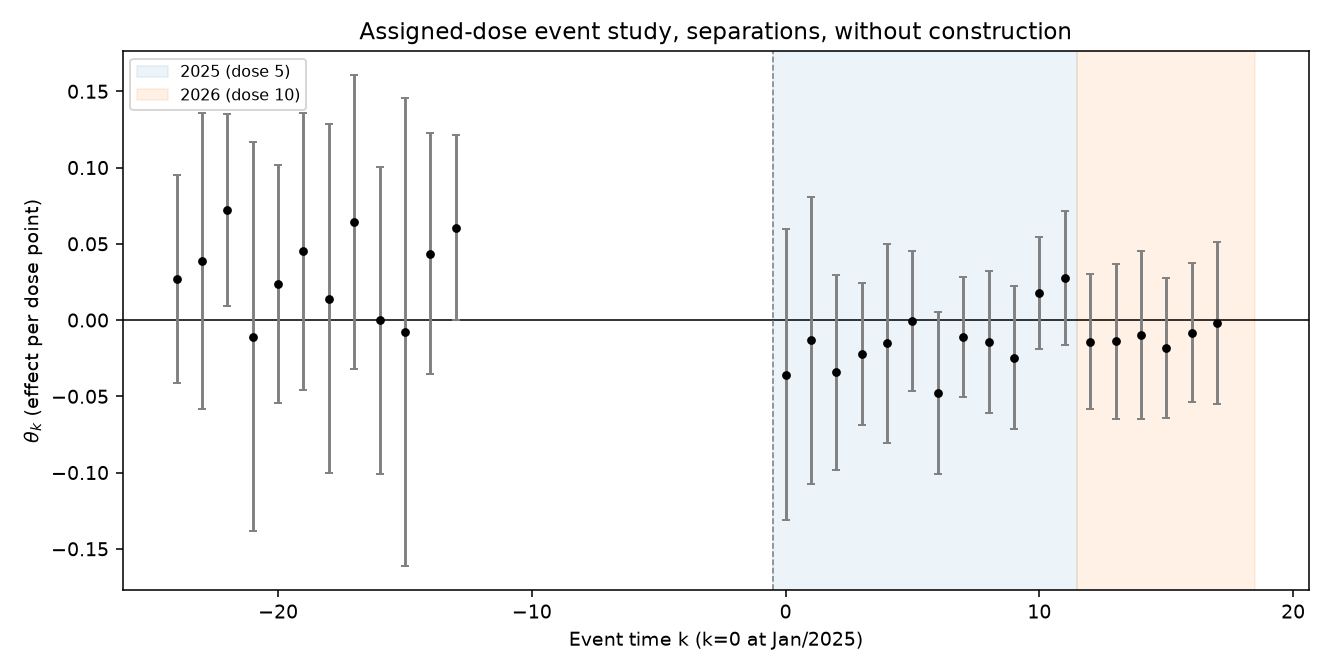
\includegraphics[width=\textwidth]{fig_es_dose_semF_base2024_desligados.png}\\
{\footnotesize semF desligados}
\end{column}
\begin{column}{0.48\textwidth}
\centering
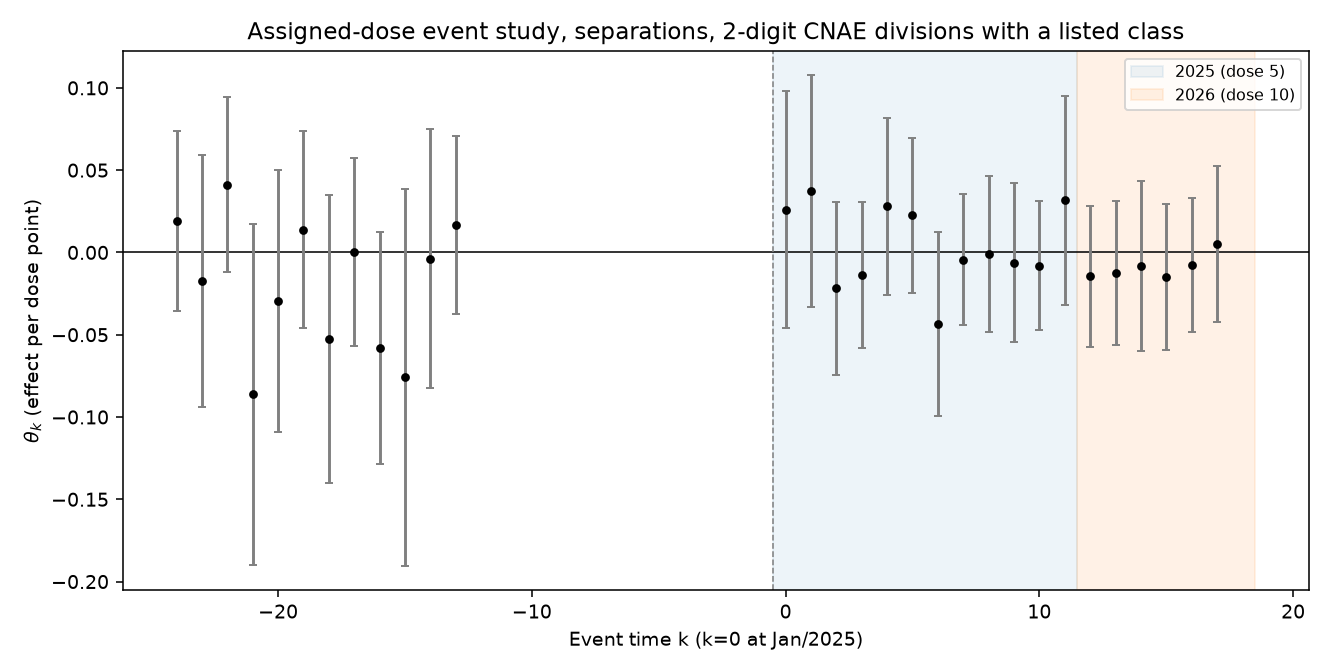
\includegraphics[width=\textwidth]{fig_es_dose_cnae2_base2024_desligados.png}\\
{\footnotesize cnae2 desligados}
\end{column}
\end{columns}
\end{frame}

\begin{frame}{BACKUP --- ES dose-\(W\) wage (rob; caveat)}
\begin{columns}[T]
\begin{column}{0.48\textwidth}
\centering
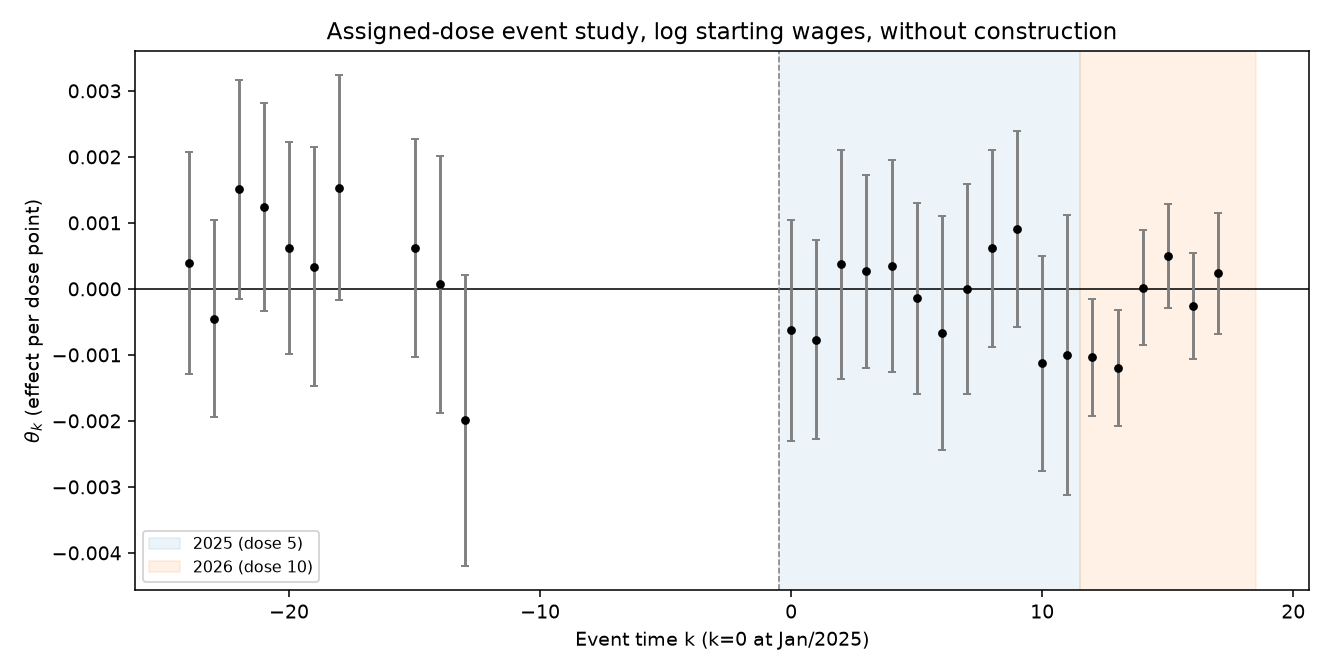
\includegraphics[width=\textwidth]{fig_es_dose_semF_base2024_log_salario.png}\\
{\footnotesize semF log salário}
\end{column}
\begin{column}{0.48\textwidth}
\centering
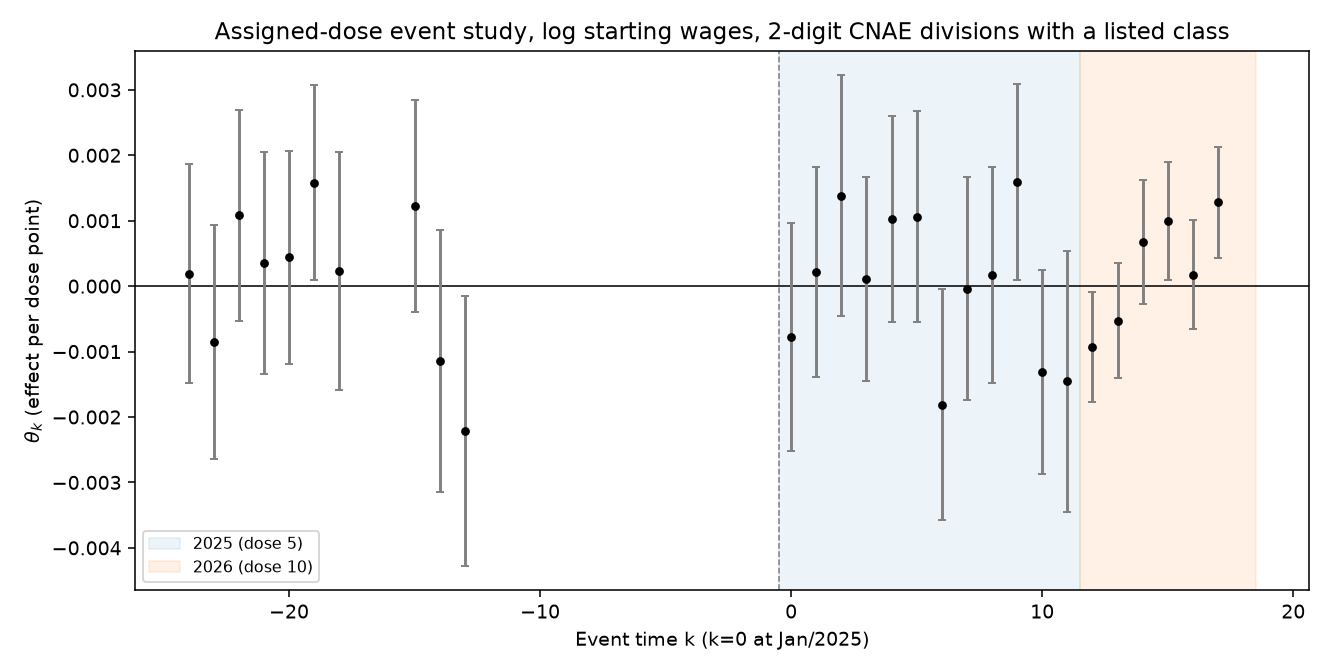
\includegraphics[width=\textwidth]{fig_es_dose_cnae2_base2024_log_salario.png}\\
{\footnotesize cnae2 log salário}
\end{column}
\end{columns}
\end{frame}

\begin{frame}{BACKUP --- ES binário saldo (rob; \(T_{\max}\))}
\begin{columns}[T]
\begin{column}{0.48\textwidth}
\centering
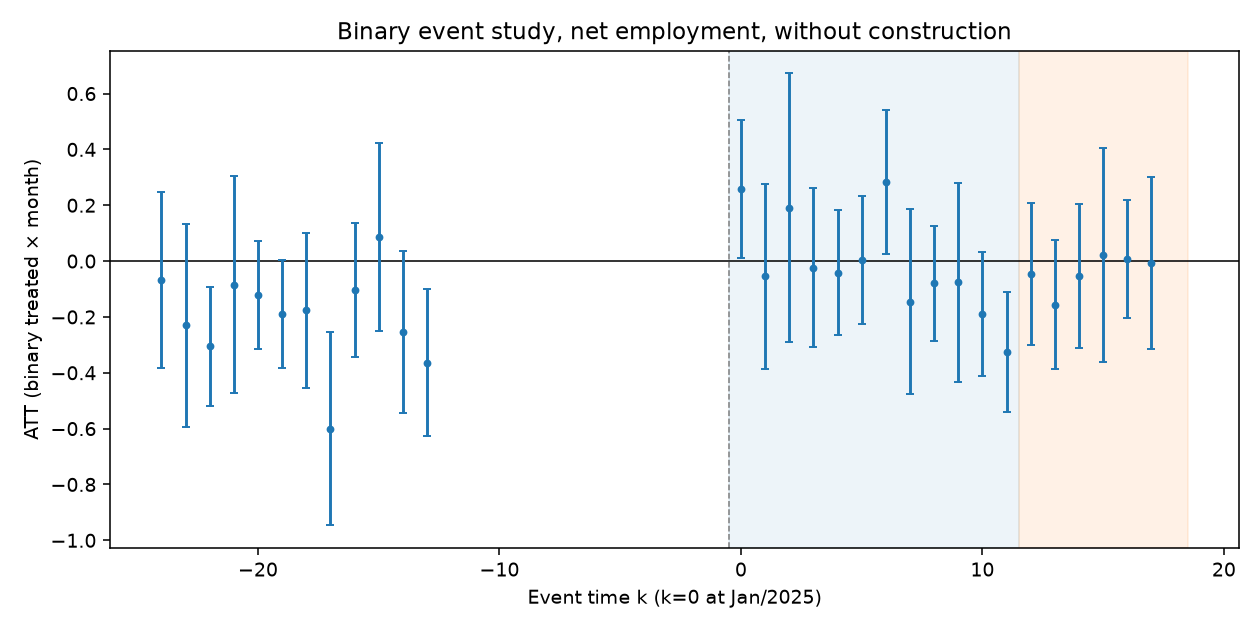
\includegraphics[width=\textwidth]{fig_es_binario_semF_base2024_saldo.png}\\
{\footnotesize semF: \(T_{\max}\approx 3.40\), \(p\approx 0.0068\) --- rejeita PT}
\end{column}
\begin{column}{0.48\textwidth}
\centering
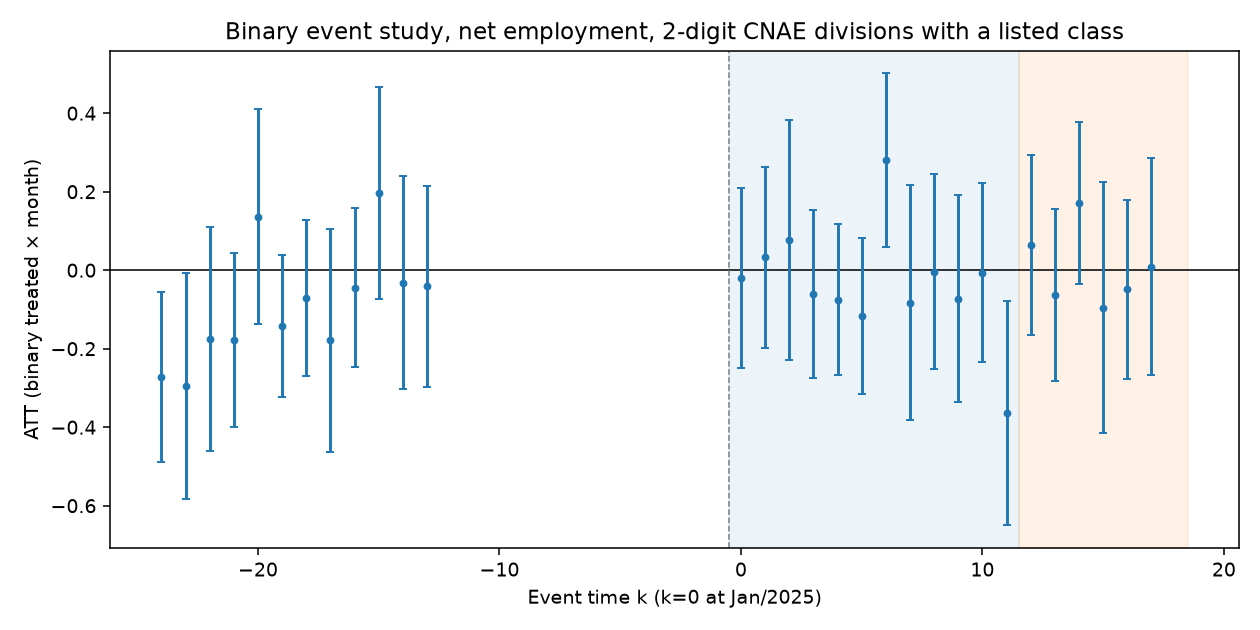
\includegraphics[width=\textwidth]{fig_es_binario_cnae2_base2024_saldo.png}\\
{\footnotesize cnae2: \(T_{\max}\approx 2.47\), \(p\approx 0.13\)}
\end{column}
\end{columns}
\end{frame}

\begin{frame}{BACKUP --- ES binário admitidos (rob)}
\begin{columns}[T]
\begin{column}{0.48\textwidth}
\centering
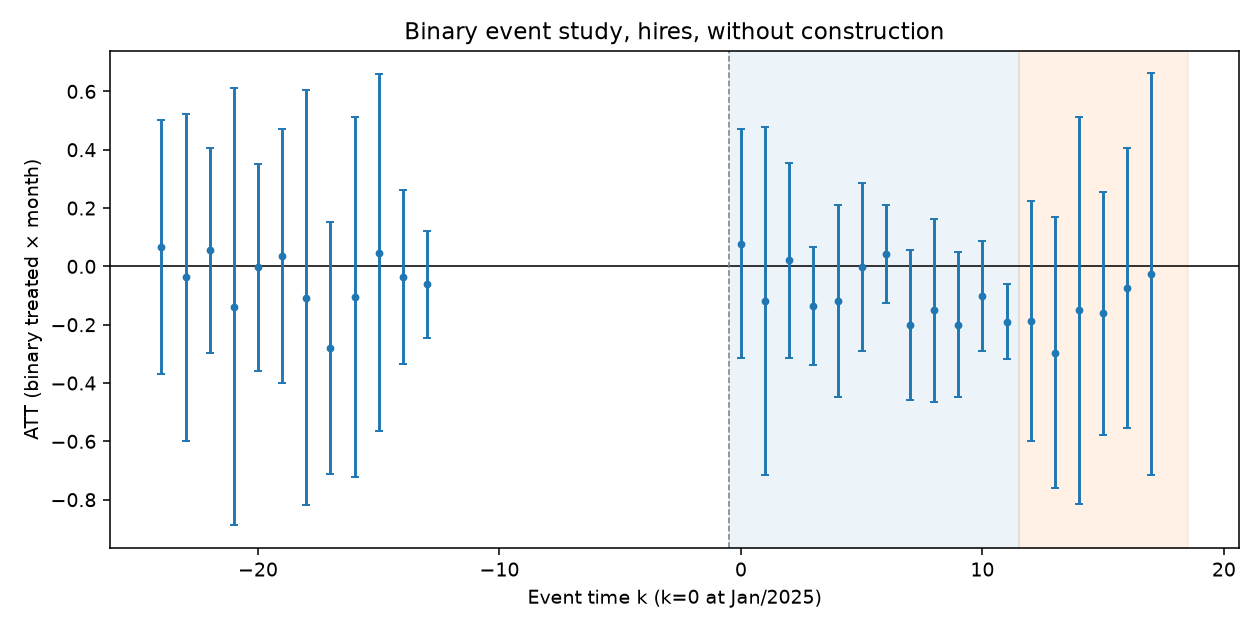
\includegraphics[width=\textwidth]{fig_es_binario_semF_base2024_admitidos.png}\\
{\footnotesize semF admitidos}
\end{column}
\begin{column}{0.48\textwidth}
\centering
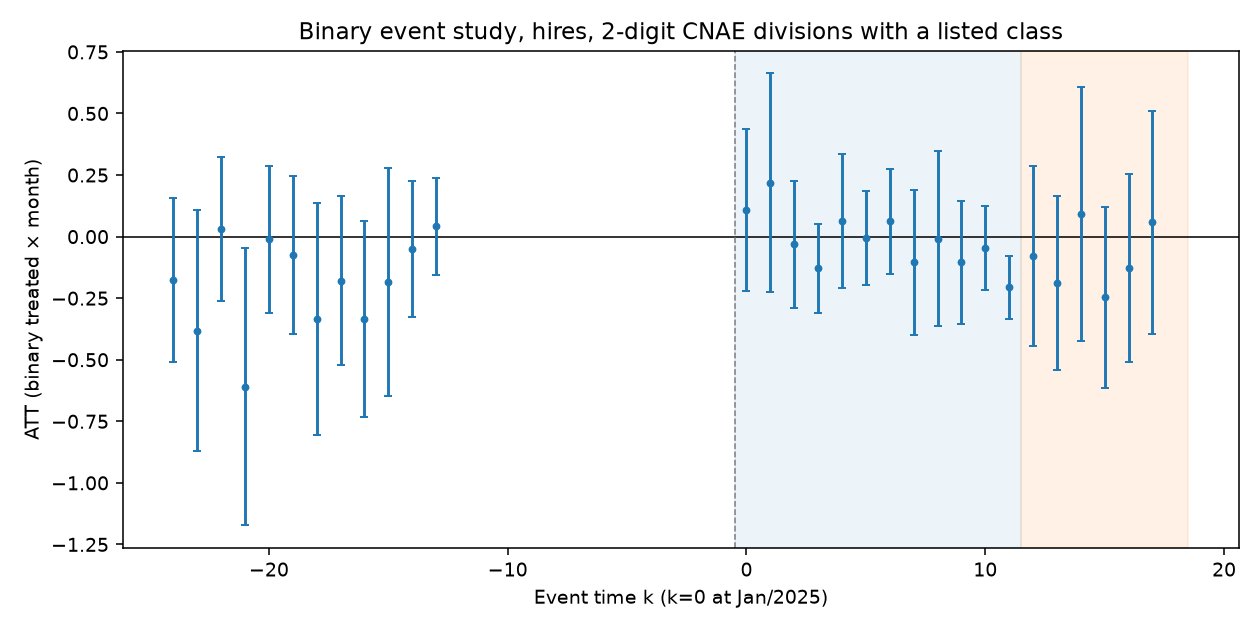
\includegraphics[width=\textwidth]{fig_es_binario_cnae2_base2024_admitidos.png}\\
{\footnotesize cnae2 admitidos}
\end{column}
\end{columns}
\end{frame}

\begin{frame}{BACKUP --- Limites}
\begin{enumerate}
  \item Efeito que só muda a forma sazonal da classe\(\times\)município pode ser absorvido por \(\alpha_{sm,c(t)}\).
  \item Janela para em jun/2026; a rampa segue até 2028.
  \item ATT setorial entre células CAGED (mistura regimes fiscais, incl.\ Simples).
  \item Lista não é aleatória: outro choque 2025--26 só nas listadas contamina o DiD.
  \item Corte semF: ATT nulo-ish mas PT usual rejeitado no ES binário do saldo --- caveat obrigatório.
\end{enumerate}
\end{frame}

\end{document}
